% Options for packages loaded elsewhere
\PassOptionsToPackage{unicode}{hyperref}
\PassOptionsToPackage{hyphens}{url}
\PassOptionsToPackage{dvipsnames,svgnames*,x11names*}{xcolor}
%
\documentclass[
  11pt,
]{article}
\usepackage{lmodern}
\usepackage{amssymb,amsmath}
\usepackage{ifxetex,ifluatex}
\ifnum 0\ifxetex 1\fi\ifluatex 1\fi=0 % if pdftex
  \usepackage[T1]{fontenc}
  \usepackage[utf8]{inputenc}
  \usepackage{textcomp} % provide euro and other symbols
\else % if luatex or xetex
  \usepackage{unicode-math}
  \defaultfontfeatures{Scale=MatchLowercase}
  \defaultfontfeatures[\rmfamily]{Ligatures=TeX,Scale=1}
\fi
% Use upquote if available, for straight quotes in verbatim environments
\IfFileExists{upquote.sty}{\usepackage{upquote}}{}
\IfFileExists{microtype.sty}{% use microtype if available
  \usepackage[]{microtype}
  \UseMicrotypeSet[protrusion]{basicmath} % disable protrusion for tt fonts
}{}
\makeatletter
\@ifundefined{KOMAClassName}{% if non-KOMA class
  \IfFileExists{parskip.sty}{%
    \usepackage{parskip}
  }{% else
    \setlength{\parindent}{0pt}
    \setlength{\parskip}{6pt plus 2pt minus 1pt}}
}{% if KOMA class
  \KOMAoptions{parskip=half}}
\makeatother
\usepackage{xcolor}
\IfFileExists{xurl.sty}{\usepackage{xurl}}{} % add URL line breaks if available
\IfFileExists{bookmark.sty}{\usepackage{bookmark}}{
\usepackage{hyperref}
}
\hypersetup{
  pdftitle={Circuits combinatoires et logique booléenne},
  pdfauthor={Première NSI Lycée du Parc},
  colorlinks=true,
  linkcolor=Maroon,
  filecolor=Maroon,
  citecolor=Blue,
  urlcolor=Blue,
  pdfcreator={LaTeX via pandoc}}
\urlstyle{same} % disable monospaced font for URLs
\usepackage[top=20mm,left=20mm,right=20mm,heightrounded]{geometry}
\usepackage{listings}
\newcommand{\passthrough}[1]{#1}
\lstset{defaultdialect=[5.3]Lua}
\lstset{defaultdialect=[x86masm]Assembler}
\usepackage{longtable,booktabs}
% Correct order of tables after \paragraph or \subparagraph
\usepackage{etoolbox}
\makeatletter
\patchcmd\longtable{\par}{\if@noskipsec\mbox{}\fi\par}{}{}
\makeatother
% Allow footnotes in longtable head/foot
\IfFileExists{footnotehyper.sty}{\usepackage{footnotehyper}}{\usepackage{footnote}}
\makesavenoteenv{longtable}
\usepackage{graphicx}
\makeatletter
\def\maxwidth{\ifdim\Gin@nat@width>\linewidth\linewidth\else\Gin@nat@width\fi}
\def\maxheight{\ifdim\Gin@nat@height>\textheight\textheight\else\Gin@nat@height\fi}
\makeatother
% Scale images if necessary, so that they will not overflow the page
% margins by default, and it is still possible to overwrite the defaults
% using explicit options in \includegraphics[width, height, ...]{}
\setkeys{Gin}{width=\maxwidth,height=\maxheight,keepaspectratio}
% Set default figure placement to htbp
\makeatletter
\def\fps@figure{htbp}
\makeatother
\setlength{\emergencystretch}{3em} % prevent overfull lines
\providecommand{\tightlist}{%
  \setlength{\itemsep}{0pt}\setlength{\parskip}{0pt}}
\setcounter{secnumdepth}{5}

\title{Circuits combinatoires et logique booléenne}
\usepackage{etoolbox}
\makeatletter
\providecommand{\subtitle}[1]{% add subtitle to \maketitle
  \apptocmd{\@title}{\par {\large #1 \par}}{}{}
}
\makeatother
\subtitle{Thèmes architectures matérielles et types de données de base}
\author{Première NSI Lycée du Parc}
\date{}

%%%jolis boites

\usepackage{fancybox, graphicx}



%%%%%%%%%%%%%%%%Packages et Macros Frederic%%%%%%%%%%%%%%%%%%%%%%%%%%%%%


%%%%Insertion de liens hypertextes %%%%

            
%%%%%%%%%%PSTricks%%%%%%%%%%%%

\usepackage{pstricks,pst-plot,pst-text,pst-tree,pst-eps,pst-fill,pst-node,pst-math,pstricks-add,pst-xkey,pst-eucl}


%%%%%%%Tikz%%%%%%%%%%%%%%%
\usepackage{pgf,tikz,tkz-tab}
% Pour les tableaux de signes ou de variations avec tkz-tab voir https://zestedesavoir.com/tutoriels/439/des-tableaux-de-variations-et-de-signes-avec-latex/#1-13389_tikz-un-package-qui-en-a-dans-le-ventre
\usetikzlibrary{arrows}
\usetikzlibrary{shapes.geometric}
\usetikzlibrary{shapes.geometric}
\usetikzlibrary{petri}
\usetikzlibrary{decorations}
\usetikzlibrary{arrows}
\usetikzlibrary{math}
 %Variables must be declared in a tikzmath environment but
       % can be used outside
%       \tikzmath{int \n; \n = 508; \x1 = 1; \y1 =1; 
%                   %computations are also possible
%                    \x2 = \x1 + 1; \y2 =\y1 +3; } 


%%%%%%%%%%%%%%%%%%%%%%%%%%%%%%%%%%%%%%%%
%%%%%%%%%%%Commandes Tikz Perso%%%%%%%%%%%%%%%

% Définition des nouvelles options xmin, xmax, ymin, ymax
% Valeurs par défaut : -3, 3, -3, 3
\tikzset{
xmin/.store in=\xmin, xmin/.default=-3, xmin=-3,
xmax/.store in=\xmax, xmax/.default=3, xmax=3,
ymin/.store in=\ymin, ymin/.default=-3, ymin=-3,
ymax/.store in=\ymax, ymax/.default=3, ymax=3,
}
% Commande qui trace la grille entre (xmin,ymin) et (xmax,ymax)
\newcommand {\grille}[2]
{\draw[help lines,black, thick] (\xmin,\ymin) grid[xstep=#1, ystep=#2] (\xmax,\ymax);}
% Commande \axes
\newcommand {\axes} {
\draw[->,very thick] (\xmin,0) -- (\xmax,0);
\draw[->,very thick] (0,\ymin) -- (0,\ymax);
\draw (0.95*\xmax, 0) node[above] {};
\draw (0, 0.95*\ymax) node[left] {};
}
% Commande qui limite l?affichage à (xmin,ymin) et (xmax,ymax)
\newcommand {\fenetre}
{\clip (\xmin,\ymin) rectangle (\xmax,\ymax);}

%Exemple d'utilisation

%\begin{center}
%\begin{tikzpicture} [xmin=-2,xmax=2,ymin=0,ymax=5]
%\grille{1} \axes \fenetre
%\draw plot[smooth] (\x,\x^2);
%\end{tikzpicture}
%\end{center}

%style pour la perspective cavalière française
%voir Tikz pour l'impatient page 68
\tikzset{math3d/.style=
{x= {(-0.353cm,-0.353cm)}, z={(0cm,1cm)},y={(1cm,0cm)}}}

%%%%%%%Symbole pour code calculatrice%%%%%%

%Flèche remplie pour défilement de menu

\newcommand{\flechefillright}{

\begin{tikzpicture}[scale=0.15] \fill (0,0)--(2,1)--(0,2)--cycle;
\end{tikzpicture}}

%%%%%%%%%%%%%Symboles pour calculatrice Casio%%%%
\newcommand{\execasio}{\Pisymbol{psy}{191}} %Retour chariot
\newcommand{\dispcasio}{\begin{pspicture}(.1,.1)\pspolygon*(.1,0)(.1,.1)\end{pspicture}} %Triangle « Disp »
\newcommand{\dispcasiotikz}{
\begin{tikzpicture}[scale=0.2]
\fill (0,0) -- (1,0) -- (1,1) -- cycle;
\end{tikzpicture}} %Triangle « Disp »
%

%Fleche entre deux lignes, d'apres 'un bon petit' : http://forum.mathematex.net/latex-f6/fleches-entre-deux-lignes-pour-resolution-d-equation-t10283.html#p99817
\newcommand\addnode[1]{\Rnode{#1}{}}
\newcommand\linknode[3]{\ncbar[angleA=0,angleB=0,nodesep=1ex,arm=10ex,offset=-2pt]{->}{#1}{#2}\Aput{\vphantom{x}#3}}


%%Commande pour touche de calculatrice

\newcommand\tc[1]{%
{
\begin{tikzpicture}
\node[draw,rectangle,rounded corners=3pt] (P) at (0,0){#1};
\end{tikzpicture}
}
}

%%%%%%%%%%%%%%%%%%%%%%%%%%%%%%%%%%%%%%%%
%%%%%%%%%%%Fin Commandes Tikz%%%%%%%%%%%%%%%


%%%%%%%%%%%%Specifiques%%%%%%%%%%%
\usepackage{wrapfig}
%pour insérer une figure à droite ou à gauche d'un texte
%\begin{wrapfigure}[nb lignes]{placement l,r,c,i(inside),o(outside)}[overhang]{width}
%ce package fonctionne mal à proximité des listes
%%%%%%%%%%%%%%%%%%%%%%%%%%%%%%%%%%%%%

%%%%%Environnements et symboles spéciaux pour faire joli%%%%%%

%%%Bclogo, pour des environnements + jolis avec insertion de logo%%%%
%Dépendances de  bclogo
\usepackage{xkeyval}  
\usepackage{etoolbox}
\usepackage{ifpdf}
\usepackage[framemethod=tikz]{mdframed}
\usepackage[tikz]{bclogo}

%\newcommand\bcpython{\includegraphics[width=17pt]{/home/fjunier/Maths/python-logo.eps}}
\newcommand\bcpython{\includegraphics[width=17pt]{/home/fjunier/Maths/python-logo.png}}
%\newcommand\bcpython{\includegraphics[width=17pt]{/home/frederic/Maths/python-logo.png}}

%% Framed
\usepackage{framed}  %Le package « framed» Crée 3 nouveaux environnements, qui se comportent comme des minipage de largeur \linewidth, mais permettant en plus de se casser entre plusieurs pages.     * framed : avec un cadre autour;     * shaded : avec un fonc coloré (il faut définir la couleur shadecolor);     * leftbar : avec une barre le long du côté gauche.

%%%%%%%%%%%%%%%%%%%Présentation de codes sources%%%%%%%%%%%%%%%%%
\usepackage{listings}
%On utilise l?environnement lstlisting pour insérer
%un code source.
%En plus de l?environnement lstlisting, on peut également utiliser la
%commande \lstinline qui fonctionne comme la commande \verb, en ce
%sens qu?on peut utiliser n?importe quel caractère comme délimiteur. Enfin,
%la commande \lstinputlisting permet de charger un code source depuis
%un fichier externe.
%Il y a deux manières de préciser des options : soit via l?option de l?envi-
%ronnement ou de la commande, soit en utilisant la commande \lstset
%qui permet de définir des options de manière globale.

\lstset{ %
  language=Python,                % the language of the code
  basicstyle=\ttfamily,           % the size of the fonts that are used for the code
  %numbers=left,                   % where to put the line-numbers
  numberstyle=\tiny,  % the style that is used for the line-numbers
  %stepnumber=2,                   % the step between two line-numbers. If it's 1, each line 
                                  % will be numbered
  %numbersep=5pt,                  % how far the line-numbers are from the code
  backgroundcolor=\color{white},      % choose the background color. You must add \usepackage{color}
  showspaces=false,               % show spaces adding particular underscores
  showstringspaces=false,         % underline spaces within strings
  showtabs=false,                 % show tabs within strings adding particular underscores
  frame=single,                   % adds a frame around the code
  rulecolor=\color{black},        % if not set, the frame-color may be changed on line-breaks within not-black text (e.g. comments (green here))
  tabsize=4,                      % sets default tabsize to 2 spaces
  captionpos=b,                   % sets the caption-position to bottom
  breaklines=true,                % sets automatic line breaking
  breakatwhitespace=false,        % sets if automatic breaks should only happen at whitespace
  %title=\lstname,                   % show the filename of files included with \lstinputlisting;
                                  % also try caption instead of title
  breakindent=1cm,
  keywordstyle=\color{blue},          % keyword style
  commentstyle=\color{red},       % comment style
  %stringstyle=\ttfamily\color{green},         % string literal style
  escapeinside={\%*}{*)},            % if you want to add LaTeX within your code
  morekeywords={*,...},              % if you want to add more keywords to the set
  deletekeywords={...}              % if you want to delete keywords from the given language
  upquote=true,columns=flexible,
xleftmargin=1cm,xrightmargin=1cm,
 inputencoding=utf8,			%Les lignes qui suivent sont pour le codage utf8
  extendedchars=true,
  literate=%
            {é}{{\'{e}}}1
            {è}{{\`{e}}}1
            {ê}{{\^{e}}}1
            {ë}{{\¨{e}}}1
            {û}{{\^{u}}}1
            {ù}{{\`{u}}}1
            {â}{{\^{a}}}1
            {à}{{\`{a} }}1
            {î}{{\^{i}}}1
            {ô}{{\^{o}}}1
            {ç}{{\c{c}}}1
            {Ç}{{\c{C}}}1
            {É}{{\'{E}}}1
            {Ê}{{\^{E}}}1
            {À}{{\`{A}}}1
            {Â}{{\^{A}}}1
            {Î}{{\^{I}}}1
}

\lstdefinestyle{rond}{
  numbers=none,
  backgroundcolor=\color{gristclair},
  frameround =tttt
}

\lstdefinestyle{compil}{
  numbers=none,
  backgroundcolor=\color{gristclair}
}
%\lstset{language=Python,basicstyle=\small , frame=single,tabsize=4,showspaces=false,showtabs=false,showstringspaces=false,numbers=left,numberstyle=\tiny , extendedchars=true}



%%%%%%%%%%%%%%%%%%%%%%%%%%%%%%%%%%%%%%%%%%%%%%%%%%%%%%%%%%%%%%%%%%%%%%%%
%%%%%%%%%%%%%%%%%%%%Environnements persos%%%%%%%%%%%%%%%%%%%%%%%%%%%%%%%%
%Syntaxe :
%\newenvironment{nom}[nombre d'args][defaut]{definitions initiales}{definitions finales}
%definitions intiales sont les commandes appelées par \begin{nom}
%Definitions finales sont les commandes appelées par \end{nom}

%%%%%%%%%%%%%%%%Définitions des environnemts persostheoreme, exemple ..%%%%
%%%% Exercice avec encadré %%%%
\newcounter{exo}
\newenvironment{exercice}[1]
{\par \medskip   \addtocounter{exo}{1} \noindent  
\begin{bclogo}[arrondi =0.1,   noborder = true, logo=\bccrayon, marge=4]{~\textbf{Exercice} \textbf{\theexo} {\itshape #1} }  \par}
{
\end{bclogo}
 \par \bigskip }

%%Axiomes, Theoremes, Propriété, Définition, Methode, Preuve


\newenvironment{axiome}[1]
{\par \medskip   \begin{leftbar} \noindent \underline{\textbf{Axiome}}\hspace{0.5cm}{\itshape #1}   \vspace*{10pt} \par }
{\end{leftbar}  \par \medskip }


\newcounter{thme}
\newenvironment{theoreme}[1]
{\par \medskip  \addtocounter{thme}{1} \noindent  
\begin{bclogo}[arrondi =0.1,  ombre = true, barre=none, logo=\bcbook, marge=4]{~\textbf{Théorème} \textbf{\thethme} {\itshape #1} }   \par}
{
\end{bclogo}
 \par \bigskip}

 \newenvironment{theoremedef}[1]
{\par \medskip   \addtocounter{thme}{1} \noindent  
\begin{bclogo}[arrondi =0.1,  ombre = true, barre=none, logo=\bcbook, marge=4]{~\textbf{Théorème-Définition} \textbf{\thethme} {\itshape #1} }   \par}
{
\end{bclogo}
 \par \bigskip }
 
\newcounter{prop}
\newenvironment{propriete}[1]
{\par \medskip   \addtocounter{prop}{1} \noindent  
\begin{bclogo}[arrondi =0.1,  ombre = true, barre=none, logo=\bcbook, marge=4]{~\textbf{Propriété} \textbf{\theprop} {\itshape #1} }   \par}
{
\end{bclogo}
 \par \bigskip }


\newenvironment{corollaire}[1]
{\par \medskip   \noindent  
\begin{bclogo}[arrondi =0.1,  ombre = true, barre=none, logo=\bcbook, marge=4]{~\textbf{Corollaire} {\itshape #1} } \par }
{
\end{bclogo}
 \par \bigskip }

\newenvironment{demo}[1]
{\par \medskip   \noindent  
\begin{bclogo}[arrondi =0.1,  ombre = true, barre=zigzag, noborder = true, logo=\bcloupe, marge=0]{~\textbf{Démonstration} {\itshape #1} } \par \vspace{10pt}}
{
\end{bclogo}
 \par \bigskip }

\newcounter{activite}
\newenvironment{activite}[1]
{\par \medskip   \noindent   \addtocounter{activite}{1}
\begin{bclogo}[arrondi =0.1,   noborder = true, logo=\bcvelo, marge=4]{~\textbf{Activité} \textbf{\theactivite} {\itshape #1} }  \par}
{
\end{bclogo}
 \par \bigskip }


\newenvironment{synthese}
{\par \medskip   \noindent   
\begin{bclogo}[arrondi =0.1,   noborder = true, logo=\bccle, marge=4]{~\textbf{Synthèse}   }  \par}
{
\end{bclogo}
 \par \bigskip }
 
 
\newcounter{rque}
\newenvironment{remarque}
{\par \medskip    \addtocounter{rque}{1} \noindent  
\begin{bclogo}[arrondi =0.1,  ombre = true, barre=snake, noborder = true, logo=\bcinfo, marge=0]{~\textbf{Remarque} \textbf{\therque}}  \par }
{
\end{bclogo}
 \par \bigskip }

\newcounter{def}
\newenvironment{definition}[1]
{\par \medskip   \addtocounter{def}{1} \noindent  
\begin{bclogo}[arrondi =0.1,  ombre = true, barre=none, logo=\bcbook, marge=4]{~\textbf{Définition} \textbf{\thedef} {\itshape #1} }  \par}
{
\end{bclogo}
 \par \bigskip }
 
 
 \newcounter{cours}
\newenvironment{cours}[1]
{\par \medskip   \addtocounter{cours}{1} \noindent  
\begin{bclogo}[arrondi =0.1,  ombre = true, barre=none, logo=\bcbook, marge=4]{~\textbf{Point de cours} \textbf{\thecours} {\itshape #1} }  \par}
{
\end{bclogo}
 \par \bigskip }
 
 

\newenvironment{introduction}
{\par \medskip    \noindent  
 \begin {bclogo}[couleur = blue!5 , arrondi =0.1,logo=\bcrosevents, marge=4] {~\textbf{Introduction}    }
 \par }
{
\end{bclogo}
 \par \bigskip }
 
\newenvironment{memo}[1]
{\par \medskip    \noindent  
\begin{bclogo}[arrondi =0.1,  ombre = true, barre=none, logo=\bccle, marge=4]{~\textbf{À retenir}  {\itshape #1} }  \par}
{
\end{bclogo}
 \par \bigskip }
 
\newcounter{exple}
\newenvironment{exemple}[1]
{\par \medskip   \addtocounter{exple}{1} \noindent  
\begin{bclogo}[arrondi =0.1,   noborder = true, logo=\bclampe, marge=4]{~\textbf{Exemple} \textbf{\theexple} {\itshape #1} }  \par}
{
\end{bclogo}
 \par \bigskip }




\newcounter{alg}
\newenvironment{algorithme}[1]
{\par \medskip   \addtocounter{alg}{1} \noindent  
 \begin {bclogo}[noborder = true, barre=zigzag,logo=\bcpython, marge=4] {~\textbf{Algorithmique} \textbf{\thealg} {\itshape #1} }  \par}
{
\end{bclogo}
 \par \bigskip }

\newcounter{prog}
\newenvironment{programme}[1]
{\par \medskip   \addtocounter{prog}{1} \noindent  
 \begin {bclogo}[noborder = true, barre=zigzag,logo=\bcpython, marge=4] {~\textbf{Programme} \textbf{\theprog} {\itshape #1} }  \par  \bigskip}
{
\end{bclogo}
 \par \bigskip }
 
\newcounter{logi}
\newenvironment{logique}[1]
{\par \medskip   \addtocounter{logi}{1} \noindent  
 \begin {bclogo}[noborder = true, barre=zigzag,logo=\bclampe, marge=4] {~\textbf{Logique} \textbf{\thelogi} {\itshape #1} }  \par}
{
\end{bclogo}
 \par \bigskip }


\newenvironment{methode}[1]
{\par \medskip    \noindent  
 \begin {bclogo}[arrondi =0.1,logo=\bcoutil, marge=4,noborder = true] {~\textbf{Méthode}   {\itshape #1} }  \par}
{
\end{bclogo}
 \par \bigskip }


\newcounter{histo}
\newenvironment{histoire}[1]
{\par \medskip   \addtocounter{histo}{1} \noindent  
 \begin {bclogo}[couleur = blue!10 , arrondi =0.1,logo=\bchorloge, marge=4] {~\textbf{Histoire} \textbf{\thehisto} {\itshape #1} }  \par}
{
\end{bclogo}
 \par \bigskip }




%Environnement contenu pour un document présentant une progression annuelle
\newenvironment{contenu}
{\par \medskip   \begin {bclogo}[ noborder = true,logo=\bccrayon] \noindent {\large \textbf{Contenu de la séance}} \vspace*{10pt} \par  }
{\end{bclogo}  \par \medskip }

%Environnement programme pour un document présentant une progression annuelle
%\newenvironment{programme}
%{\par \medskip   \begin {bclogo}[ noborder = true, barre=zigzag,logo=\bcinfo] \noindent {\large \textbf{Programme officiel}} \vspace*{10pt} \par  }
%{\end{bclogo}  \par \medskip }

%Environnement programme pour un document présentant une progression annuelle
\newenvironment{ressource}
{\par \medskip   \begin {bclogo}[ noborder = true,logo=\bcbook] \noindent {\large \textbf{Ressources}}\\vspace*{10pt} \par }
{\end{bclogo}  \par \medskip }




%%%%%%%%%%%%%%%%%%Maths divers%%%%%%%%%%%%%%%%%%%%%%%%%
%%%%%%%%%%%%%Nombres%%%%%%%%%%%%%%%%

%Ensemble prive de...
%\newcommand{\prive}{\boi}%{\backslash}

%Ensembles de nombres%%%%%%%%%%%%%%%%%
\newcommand{\R}{\mathbb{R}}
\newcommand{\N}{\mathbb{N}}
\newcommand{\D}{\mathbb{D}}
\newcommand{\Z}{\mathbb{Z}}
\newcommand{\Q}{\mathbb{Q}}
%\newcommand{\C}{\mathbb{C}}
\newcommand{\df}{~\ensuremath{]0;+\infty[}~}
\newcommand{\K}{\mathbb{K}}

%%%%%%%%Arithmetique%%%%%%%%%%
%PGCD, PPCM
\newcommand{\PGCD}{\mathop{\rm PGCD}\nolimits}
\newcommand{\PPCM}{\mathop{\rm PPCM}\nolimits}

%Intervalles
\newcommand{\interoo}[2]{]#1\, ;\, #2[}
\newcommand{\Interoo}[2]{\left]#1\, ;\, #2\right[}
\newcommand{\interof}[2]{]#1\, ;\, #2]}
\newcommand{\Interof}[2]{\left]#1\, ;\, #2\right]}
\newcommand{\interfo}[2]{[#1\, ;\, #2[}
\newcommand{\Interfo}[2]{\left[#1\, ;\, #2\right[}
\newcommand{\interff}[2]{[#1\, ;\, #2]}
\newcommand{\Interff}[2]{\left[#1\, ;\, #2\right]}
%\newcommand\interentiers #1#2{[\! [#1\, ;\, #2]\! ]}
\newcommand{\interentiers}[2]{\llbracket #1\, ;\, #2\rrbracket}
%


%%%%%%%%%%%%%%Nombres complexes%%%%%

\newcommand{\ic}{\text{i}}
%\newcommand{\I}{\text{i}}
\newcommand{\im}[1]{\text{Im}\left(#1\right)}
\newcommand{\re}[1]{\text{Re}\left(#1\right)}
\newcommand{\Arg}[1]{\text{arg}\left(#1\right)}
\newcommand{\Mod}[1]{\left[#1\right]}
%Parties entière, réelle, imaginaire, nombre i
\newcommand{\ent}[1]{\text{E}\left(#1\right)}
\renewcommand{\Re}{\mathop{\rm Re}\nolimits}
\renewcommand{\Im}{\mathop{\rm Im}\nolimits}
\renewcommand{\i}{\textrm{i}}

%%%%%%%%%%%Probabilites et statistiques%%%%%
\newcommand{\loibinom}[2]{\mathcal{B}\left(#1\ ; \ #2 \right)}
\newcommand{\loinorm}[2]{\mathcal{N}\left(#1\ ; \ #2 \right)}
\newcommand{\loiexp}[1]{\mathcal{E}\left(#1\right)}
\newcommand{\proba}[1]{\mathbb{P}\big(#1\big)}
\newcommand{\probacond}[2]{\mathbb{P}_{#2}\big(#1\big)}
\newcommand{\esperance}[1]{\mathbb{E}\left(#1\right)}
\newcommand{\variance}[1]{\mathbb{V}\left(#1\right)}
\newcommand{\ecart}[1]{\sigma\left(#1\right)}
\newcommand{\dnormx}{\frac{1}{\sqrt{2\pi}} \text{e}^{-\frac{x^2}{2}}}
\newcommand{\dnormt}{\frac{1}{\sqrt{2\pi}} \text{e}^{-\frac{t^2}{2}}}

%Covariance
\newcommand{\cov}{\mathop{\rm cov}\nolimits}
%


%%%%%%%%%%Analyse%%%%%%%%%%%

%%%%%%%%%%%Courbe%%%%%%%%%%%%
\newcommand{\courbe}[1]{\ensuremath{\mathcal{C}_{#1}}}

%%%%%%%Fonction exponentielle%%%%%
\newcommand{\fe}{~fonction exponentielle~}
\newcommand{\e}{\text{e}}

%Fonction cotangente
\newcommand{\cotan}{\mathop{\rm cotan}\nolimits}
%%%%%%%%%%%%%%%%%%%%%%%%%%%%%%%%%%%%%%%%%
%
%Fonctions hyperboliques
\newcommand{\ch}{\mathop{\rm ch}\nolimits}
\newcommand{\sh}{\mathop{\rm sh}\nolimits}


%%%%%%%%%%%%%%Limites%%%%%%
\newcommand{\limite}[2]{\lim\limits
_{x \to #1} #2}
\newcommand{\limitesuite}[1]{\lim\limits
_{n \to +\infty} #1}
\newcommand{\limiteg}[2]{\lim\limits
_{\substack{x \to #1 \\ x < #1 }} #2}
\newcommand{\limited}[2]{\lim\limits
_{\substack{x \to #1 \\ x > #1 }} #2}

%%%%%%%%%%Continuité%%%%%%%%%%%
\newcommand{\TVI}{théorème des valeurs intermédiaires}

%%%%%%%%%%%Suites%%%%%%%%%%%%
\newcommand{\suite}[1]{\ensuremath{\left(#1_{n}\right)}}
\newcommand{\Suite}[2]{\ensuremath{\left(#1\right)_{#2}}}
%

%%%%%%%%%%%%%%%Calcul intégral%%%%%%
\newcommand{\dx}{\ensuremath{\text{d}x}}		% dx
\newcommand{\dt}{\ensuremath{\text{d}t}}		% dt
\newcommand{\dtheta}{\ensuremath{\text{d}\theta}}		% dtheta
\newcommand{\dy}{\ensuremath{\text{d}y}}		% dy
\newcommand{\dq}{\ensuremath{\text{d}q}}		% dq

%%%Intégrale%%%
\newcommand{\integralex}[3]{\int_{#1}^{#2} #3 \ \dx}
\newcommand{\integralet}[3]{\int_{#1}^{#2} #3 \ \dt}
\newcommand{\integraletheta}[3]{\int_{#1}^{#2} #3 \ \dtheta}

%%%%%Equivalent%%
\newcommand{\equivalent}[1]{\build\sim_{#1}^{}}

%o et O%%%%
\renewcommand{\o}[2]{\build o_{#1\to #2}^{}}
\renewcommand{\O}[2]{\build O_{#1\to #2}^{}}



%%%%%%%%%%%%%%%Geometrie%%%%%%%%%%%%%%%%%%%%%%%

%%%%%%%%%%%%%%%Reperes%%%%%%%%%%%%%%
\def\Oij{\ensuremath{\left(\text{O},~\vect{\imath},~\vect{\jmath}\right)}}
\def\Oijk{\ensuremath{\left(\text{O},~\vect{\imath},~ \vect{\jmath},~ \vect{k}\right)}}
\def\Ouv{\ensuremath{\left(\text{O},~\vect{u},~\vect{v}\right)}}
\renewcommand{\ij}{(\vec\imath\, ;\vec\jmath\,)}
\newcommand{\ijk}{(\vec\imath\, ;\vec\jmath\, ;\vec k\,)}
\newcommand{\OIJ}{(O\,;\, I\,;\, J\,)}
\newcommand{\repere}[3]{\big(#1\, ;\,\vect{#2} ;\vect{#3}\big)}
\newcommand{\reperesp}[4]{\big(#1\, ;\,\vect{#2} ;\vect{#3} ;\vect{#4}\big)}

%%%%%%%%%Coordonnees%%%%%%%%%%%%%%
\newcommand{\coord}[2]{(#1\, ;\, #2)}
\newcommand{\bigcoord}[2]{\big(#1\, ;\, #2\big)}
\newcommand{\Coord}[2]{\left(#1\, ;\, #2\right)}
\newcommand{\coordesp}[3]{(#1\, ;\, #2\, ;\, #3)}
\newcommand{\bigcoordesp}[3]{\big(#1\, ;\, #2\, ;\, #3\big)}
\newcommand{\Coordesp}[3]{\left(#1\, ;\, #2\, ;\, #3\right)}
\newcommand{\Vcoord}[3]{\begin{pmatrix} #1 \\ #2 \\ #3 \end{pmatrix}}
%Symboles entre droites
%\newcommand{\paral}{\sslash}
\newcommand{\paral}{\mathop{/\!\! /}}
%

%%%%%%%%%Produit scalaire, Angles%%%%%%%%%%
\newcommand{\scal}[2]{\vect{#1} \, \cdot \, \vect{#2}}
\newcommand{\Angle}[2]{\left(\vect{#1} \, , \, \vect{#2}\right)}
\newcommand{\Anglegeo}[2]{\left(\widehat{\vect{#1} \, ; \, \vect{#2}}\right)}
\renewcommand{\angle}[1]{\widehat{#1}}
\newcommand{\anglevec}[2]{\left(\vect {#1}\, ,\,\vect {#2} \right)}
\newcommand{\anglevecteur}[2]{(#1\, , \, #2)}
\newcommand{\Anglevec}[2]{(\vecteur{#1}\, ,\,\vecteur{#2})}
\newcommand{\prodscal}[2]{#1 \, \cdot \, #2}
%


%Arc
%\newcommand{\arc}[1]{\wideparen{#1}}
\newcommand{\arcoriente}[1]{\overset{\curvearrowright}{#1}}
%
%


%%%%%%%%%%%%%%%Normes%%%%%%%%%%%%%%%%
\newcommand{\norme}[1]{\left\| #1\right\|}
\newcommand{\normebis}[1]{\delim{2pt}{\|}{9pt}\! #1\delim{2pt}{\|}{9pt}}
\newcommand{\normetriple}[1]{\left |\kern -.07em\left\| #1\right |\kern -.07em\right\|}
\newcommand{\valabs}[1]{\big| \, #1 \, \big|}
%

%%%%%%%%%%%%%%%%%%%%%%%%%%%Degré%%%%%%
%\newcommand{\Degre}{\ensuremath{^\circ}}
%La commande \degre est déjà définie dans le package babel

%%%%%%%%%%Vecteurs%%%%%%%%%%%
\newcommand{\vect}[1]{\mathchoice%
{\overrightarrow{\displaystyle\mathstrut#1\,\,}}%
{\overrightarrow{\textstyle\mathstrut#1\,\,}}%
{\overrightarrow{\scriptstyle\mathstrut#1\,\,}}%
{\overrightarrow{\scriptscriptstyle\mathstrut#1\,\,}}}



%%%%%%%%%%%%%Algebre%%%%%%%%%%%%%%%


%%%%%%%%%%Systemes%%%%%%%%%%%
%Systemes
\newcommand{\sys}[2]{
\left\lbrace
 \begin{array}{l}
  \negthickspace\negthickspace #1\\
  \negthickspace\negthickspace #2\\
 \end{array}
\right.\negthickspace\negthickspace}
\newcommand{\Sys}[3]{
\left\lbrace
 \begin{array}{l}
  #1\\
  #2\\
  #3\\
 \end{array}
\right.}
\newcommand{\Sysq}[4]{
\left\lbrace
 \begin{array}{l}
  #1\\
  #2\\
  #3\\
  #4\\
 \end{array}
\right.}
%
%

%%%%%%%%%%%%%%%%Matrices%%%%%%%%%%%%%%%%%%
%Comatrice
\newcommand{\com}{\mathop{\rm com}\nolimits}
%
%
%Trace
\newcommand{\tr}{\mathop{\rm tr}\nolimits}
%
%
%Transposee
\newcommand{\transposee}[1]{{\vphantom{#1}}^t\negmedspace #1}
%
%
%Noyau
\newcommand{\Ker}{\mathop{\rm Ker}\nolimits}
%
%

%
%Matrices
\newcommand{\Mn}{\mathcal M_n}
\newcommand{\matrice}[4]{
\left(
 \begin{array}{cc}
  #1 & #2 \\
  #3 & #4
 \end{array}
\right)}

\newcommand{\Matrice}[9]{
\left(
 \begin{array}{ccc}
  #1 & #2 & #3\\
  #4 & #5 & #6\\
  #7 & #8 & #9
 \end{array}
\right)}
\newcommand{\Vect}[3]{
\left(\negmedspace
 \begin{array}{c}
  #1\\
  #2\\
  #3
 \end{array}\negmedspace
\right)}
\newcommand{\Ideux}{\matrice{1}{0}{0}{1}}
\newcommand{\Itrois}{\Matrice{1}{0}{0}{0}{1}{0}{0}{0}{1}}
%
%
%Determinants
\newcommand{\determinant}[4]{
\left|
 \begin{array}{cc}
  #1 & #2 \\
  #3 & #4
 \end{array}
\right|}
\newcommand{\Determinant}[9]{
\left|
 \begin{array}{ccc}
  #1 & #2 & #3\\
  #4 & #5 & #6\\
  #7 & #8 & #9
 \end{array}
\right|}

\begin{document}
\maketitle

\renewcommand*\contentsname{Table des matières}
{
\hypersetup{linkcolor=}
\setcounter{tocdepth}{3}
\tableofcontents
}
\hypertarget{cruxe9dits}{%
\section*{Crédits}\label{cruxe9dits}}
\addcontentsline{toc}{section}{Crédits}

\emph{Ce cours est largement inspiré du chapitre 22 du manuel NSI de la
collection Tortue chez Ellipsen auteurs : Ballabonski, Conchon,
Filliatre, N'Guyen.}

\hypertarget{pruxe9ambule}{%
\section*{Préambule}\label{pruxe9ambule}}
\addcontentsline{toc}{section}{Préambule}

Les circuits d'un ordinateur manipulent uniquement des 0 ou des 1
représentés en interne par des tensions hautes ou basses. Les premiers
ordinateurs construits dans la période 1945-1950 sont basés sur une
technologie de tube à vide ou tube électrique. En 1947, aux laboratoires
Bell, \href{https://fr.wikipedia.org/wiki/Transistor}{Shockley, Bardeen
et Brattain} inventent le \textbf{transistor} au \emph{germanium} un
petit composant électronique qui se comporte comme un interrupteur. Les
transistors, plus petits et dissipant moins de chaleur, vont supplanter
les tubes électriques : en 1954 le \emph{germanium} est remplacé par le
\emph{silicium}, en 1955 apparaissent les premiers ordinateurs
entièrement transistorisés, en 1960 le transistor à effet de champ
permet l'intégration de dizaines composants dans un centimètre carré.
Les transistors sont ensuite directement gravés dans une plaque de
\emph{silicium} constituant un \textbf{cicrcuit intégré}. En 1965 Gordon
Moore futur directeur d'Intel énonce la
\href{https://fr.wikipedia.org/wiki/Loi_de_Moore}{loi empirique} portant
son nom qui fixe une feuille de route à l'industrie des
mircroprocesseurs : le doublement de la densité d'intégration des
transistors tous les deux ans. Cette loi s'est vérifiée jusqu'à présent
avec une finesse de gravure d'environ 5 nanomètres en 2020. Le
\href{https://en.wikipedia.org/wiki/Moore\%27s_law\#/media/File:Moore's_Law_Transistor_Count_1971-2018.png}{graphique}
ci-dessous représente l'évolution du nombre de transistors par circuit
intégré.

\begin{center}{}

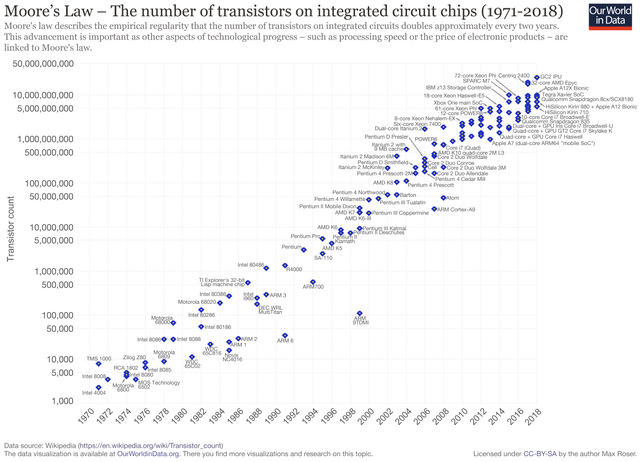
\includegraphics[width=0.9\textwidth,height=\textheight]{images/640px-Moores_Law_Transistor_Count_1971-2018.png}\\

\end{center}

\hypertarget{portes-logiques}{%
\section{Portes logiques}\label{portes-logiques}}

\hypertarget{le-transistor-porte-logique-de-base}{%
\subsection{Le transistor porte logique de
base}\label{le-transistor-porte-logique-de-base}}

\begin{definition}{}

Un \textbf{transistor} possède trois broches : la grille, la sortie (ou
drain) et la source soumis à des états de tension haute ou basse qu'on
peut assimiler aux valeurs binaires 1 et 0 d'un \textbf{bit}. Si la
tension appliquée sur la grille est haute (bit à 1) alors le transitor
laisse passer le courant entre la source d'énergie et la sortie et cette
dernière passe à l'état de tension basse (bit à 0), sinon la sortie
reste en tension haute (bit 1).

Une \textbf{fonction logique} prend un ou plusieurs bits en entrée et
retourne un ou plusieurs bits en sortie. Une \textbf{porte logique} est
un circuit électronique représentant une \textbf{fonction logique}.

Une \textbf{table logique} représente les sorties produites par une
fonction logique pour toutes les entrées possibles.

Un transistor représente une fonction logique dont le bit d'entrée est
l'état de tension de la grille et le bit de sortie, l'état de tension de
la sortie. La \textbf{table logique} (table 1) associée est celle du
\textbf{NON logique} ou \textbf{Inverseur}.

Fichier de test \href{http://www.cburch.com/logisim/}{Logisim} :
\href{circuits_logisim/transistor.circ}{transistor.circ}.

\end{definition}

\begin{center}{}

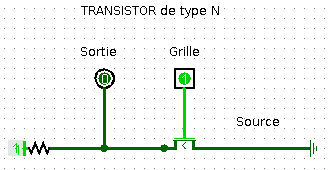
\includegraphics[width=0.5\textwidth,height=\textheight]{images/transistor.png}\\

\end{center}

\begin{longtable}[]{@{}cl@{}}
\caption{\textbf{Table logique d'une porte NON}}\tabularnewline
\toprule
A & B = NON(A)\tabularnewline
\midrule
\endfirsthead
\toprule
A & B = NON(A)\tabularnewline
\midrule
\endhead
0 & 1\tabularnewline
1 & 0\tabularnewline
\bottomrule
\end{longtable}

\textbf{Il existe deux conventions de représentation symbolique des
portes logiques, une européenne et une américaine.}

\begin{center}

\begin{tabular}{cc}

\begin{minipage}{0.5\linewidth}

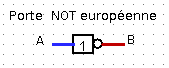
\includegraphics{images/porte_not_european.png}\\

\end{minipage} &

\begin{minipage}{0.5\linewidth}

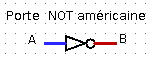
\includegraphics{images/porte_not_american.png}\\

\end{minipage} \end{tabular}

\end{center}

\href{videos/transistor-definition1.mp4}{Tutoriel video Logisim : le
transistor}

\hypertarget{dautres-portes-logiques}{%
\subsection{D'autres portes logiques}\label{dautres-portes-logiques}}

\hypertarget{transistors-en-suxe9rie-ou-en-paralluxe8le}{%
\subsubsection{Transistors en série ou en
parallèle}\label{transistors-en-suxe9rie-ou-en-paralluxe8le}}

\begin{exercice}{}

On donne ci-dessous les représentations de deux portes logiques :

\begin{itemize}
\tightlist
\item
  La \textbf{porte NAND} constituée de deux transistors en série
\item
  La \textbf{porte NOR} constituée de deux transistors en parallèle
\end{itemize}

Chacune de ces portes logiques comportent deux bits d'entrée : A pour la
grille du transistor 1 et B pour la grille du transistor 2 et un bit de
sortie.

Compléter leurs tables logiques.

Vérifier avec \href{http://www.cburch.com/logisim/}{Logisim} et les
fichiers \href{circuits_logisim/porte_NAND.circ}{porte\_NAND.circ} et
\href{circuits_logisim/porte_NOR.circ}{porte\_NOR.circ}.

\href{videos/porteNAND.mp4}{Tutoriel video Logisim : porte NAND}

\href{videos/porteNOR.mp4}{Tutoriel video Logisim : porte NOR}

\begin{longtable}[]{@{}cll@{}}
\toprule
A & B & NAND(A, B)\tabularnewline
\midrule
\endhead
0 & 0 &\tabularnewline
0 & 1 &\tabularnewline
1 & 0 &\tabularnewline
1 & 1 &\tabularnewline
\bottomrule
\end{longtable}

\begin{longtable}[]{@{}cll@{}}
\toprule
A & B & NOR(A, B)\tabularnewline
\midrule
\endhead
0 & 0 &\tabularnewline
0 & 1 &\tabularnewline
1 & 0 &\tabularnewline
1 & 1 &\tabularnewline
\bottomrule
\end{longtable}

\end{exercice}

\begin{center}

\begin{tabular}{cc}

\begin{minipage}{0.5\linewidth}

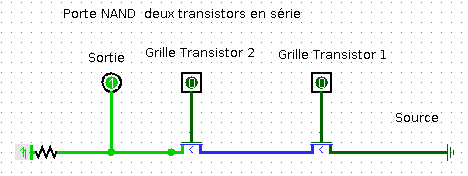
\includegraphics[width=0.8\textwidth,height=\textheight]{images/porte_nand.png}\\

\end{minipage} &

\begin{minipage}{0.5\linewidth}

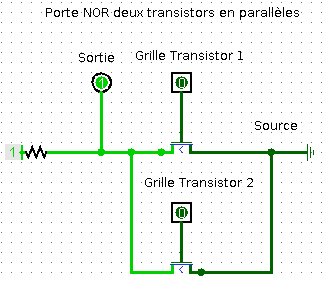
\includegraphics[width=0.8\textwidth,height=\textheight]{images/porte_nor.png}\\

\end{minipage} \end{tabular}

\end{center}

\textbf{Voici les représentations symboliques des portes logiques NAND
et NOR :}

\begin{center}

\begin{tabular}{cc}

\begin{minipage}{0.5\linewidth}

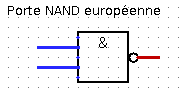
\includegraphics{images/porte_nand_european.png}\\

\end{minipage} &

\begin{minipage}{0.5\linewidth}

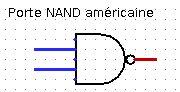
\includegraphics{images/porte_nand_american.png}\\

\end{minipage} \end{tabular}

\end{center}

\begin{center}

\begin{tabular}{cc}

\begin{minipage}{0.5\linewidth}

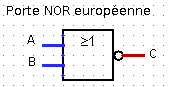
\includegraphics{images/porte_nor_european.png}\\

\end{minipage} &

\begin{minipage}{0.5\linewidth}

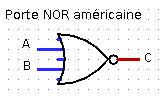
\includegraphics{images/porte_nor_american.png}\\

\end{minipage} \end{tabular}

\end{center}

\hypertarget{portes-logiques-et-fonctions-logiques-uxe9luxe9mentaires}{%
\subsubsection{Portes logiques et fonctions logiques
élémentaires}\label{portes-logiques-et-fonctions-logiques-uxe9luxe9mentaires}}

\begin{exercice}{}

Fichier de test \href{http://www.cburch.com/logisim/}{Logisim} :
\href{circuits_logisim/exercice2.circ}{exercice2.circ}.

\begin{enumerate}
\def\labelenumi{\arabic{enumi}.}
\tightlist
\item
  Compléter la table logique de la porte logique représentée par le
  circuit ci-dessous. Quelle porte logique peut-on ainsi représenter ?
\end{enumerate}

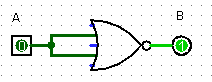
\includegraphics{images/porte_not_with_nor.png}\\

\begin{longtable}[]{@{}cl@{}}
\toprule
A & B = f(A)\tabularnewline
\midrule
\endhead
0 &\tabularnewline
1 &\tabularnewline
\bottomrule
\end{longtable}

\begin{enumerate}
\def\labelenumi{\arabic{enumi}.}
\setcounter{enumi}{1}
\tightlist
\item
  Compléter la table logique de la porte logique représentée par le
  circuit ci-dessous. Quelle fonction logique correspond à cette porte
  logique ?
\end{enumerate}

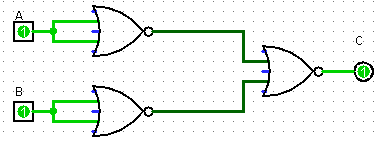
\includegraphics[width=0.6\textwidth,height=\textheight]{images/porte_and_with_nor.png}\\

\begin{longtable}[]{@{}cll@{}}
\toprule
A & B & C = g(A, B)\tabularnewline
\midrule
\endhead
0 & 0 &\tabularnewline
0 & 1 &\tabularnewline
1 & 0 &\tabularnewline
1 & 1 &\tabularnewline
\bottomrule
\end{longtable}

\href{videos/exercice2.mp4}{Tutoriel video Logisim : exercice 2}

\end{exercice}

\begin{exercice}{}

Fichier de test \href{http://www.cburch.com/logisim/}{Logisim} :
\href{circuits_logisim/exercice3.circ}{exercice3.circ}.

\begin{enumerate}
\def\labelenumi{\arabic{enumi}.}
\tightlist
\item
  Compléter la table logique de la porte logique représentée par le
  circuit ci-dessous. Quelle porte logique peut-on ainsi représenter ?
\end{enumerate}

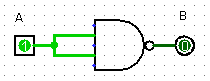
\includegraphics{images/porte_not_with_nand.png}\\

\begin{longtable}[]{@{}cl@{}}
\toprule
A & B = f(A)\tabularnewline
\midrule
\endhead
0 &\tabularnewline
1 &\tabularnewline
\bottomrule
\end{longtable}

\begin{enumerate}
\def\labelenumi{\arabic{enumi}.}
\setcounter{enumi}{1}
\tightlist
\item
  Compléter la table logique de la porte logique représentée par le
  circuit ci-dessous. Quelle fonction logique correspond à cette porte
  logique ?
\end{enumerate}

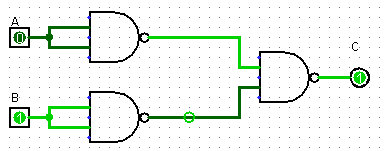
\includegraphics[width=0.6\textwidth,height=\textheight]{images/porte_or_with_nand.png}\\

\begin{longtable}[]{@{}cll@{}}
\toprule
A & B & C = g(A, B)\tabularnewline
\midrule
\endhead
0 & 0 &\tabularnewline
0 & 1 &\tabularnewline
1 & 0 &\tabularnewline
1 & 1 &\tabularnewline
\bottomrule
\end{longtable}

\href{videos/exercice3.mp4}{Tutoriel video Logisim : exercice 3}

\end{exercice}

\textbf{Voici les représentations symboliques des portes logiques
\passthrough{\lstinline!AND!} et \passthrough{\lstinline!OR!} :}

\begin{center}

\begin{tabular}{cc}

\begin{minipage}{0.5\linewidth}

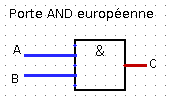
\includegraphics{images/porte_and_european.png}\\

\end{minipage} &

\begin{minipage}{0.5\linewidth}

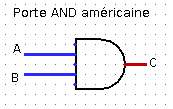
\includegraphics{images/porte_and_american.png}\\

\end{minipage} \end{tabular}

\end{center}

\begin{center}

\begin{tabular}{cc}

\begin{minipage}{0.5\linewidth}

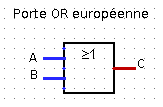
\includegraphics{images/porte_or_european.png}\\

\end{minipage} &

\begin{minipage}{0.5\linewidth}

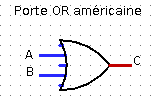
\includegraphics{images/porte_or_american.png}\\

\end{minipage} \end{tabular}

\end{center}

\begin{exercice}{}

\begin{enumerate}
\def\labelenumi{\arabic{enumi}.}
\tightlist
\item
  Construire un circuit représentant une porte
  \passthrough{\lstinline!OR!} uniquement avec des portes
  \passthrough{\lstinline!NOR!}.
\item
  Construire un circuit représentant une porte
  \passthrough{\lstinline!AND!} uniquement avec des portes
  \passthrough{\lstinline!NAND!}.
\end{enumerate}

Ainsi chacune des portes, \passthrough{\lstinline!NAND!} ou
\passthrough{\lstinline!NOR!} permet de construire les portes
\passthrough{\lstinline!NOT!}, \passthrough{\lstinline!OR!},
\passthrough{\lstinline!AND!}. Toute porte logique pouvant s'exprimer à
l'aide de ces trois portes, les portes \passthrough{\lstinline!NAND!} et
\passthrough{\lstinline!NOR!} sont dites \emph{universelles}.

\href{videos/exercice4.mp4}{Tutoriel video Logisim : exercice 4}

\end{exercice}

\hypertarget{fonctions-booluxe9ennes}{%
\section{Fonctions booléennes}\label{fonctions-booluxe9ennes}}

\hypertarget{fonctions-booluxe9ennes-1}{%
\subsection{Fonctions booléennes}\label{fonctions-booluxe9ennes-1}}

\begin{definition}{}

\begin{itemize}
\tightlist
\item
  Un \textbf{booléen} est un type de données pouvant prendre deux
  valeurs \passthrough{\lstinline!True!} (Vrai) ou
  \passthrough{\lstinline!False!} (Faux) qu'on représente numériquement
  par un \textbf{bit} de valeur \(1\) pour
  \passthrough{\lstinline!True!} ou \(0\) pour
  \passthrough{\lstinline!False!}. Electroniquement, les valeurs 1 et 0
  se traduisent respectivement par des tensions haute ou basse.
\item
  Une \textbf{fonction booléenne} \(f\) associe un booléen à un ou
  plusieurs booléens.
\item
  Une \textbf{fonction booléenne} avec \(n\) arguments est définie sur
  un ensemble \(\{0;1\}^n\) à \(2^n\) valeurs et prend ses valeurs dans
  \(\{0;1\}\) qui a \(2\) éléments. On peut recenser les \(2^n\)
  évaluations d'une fonction booléenne à \(n\) arguments dans une
  \textbf{table de vérité} qui la définit entièrement. Il existe
  \(2^{2^n}\) fonctions booléennes à \(n\) arguments.
\item
  Une \textbf{porte logique} est la représentation sous forme de circuit
  d'une fonction booléenne et sa \textbf{table logique} est la
  \textbf{table de vérité} de cette fonction.
\end{itemize}

\end{definition}

\begin{exercice}{}

\begin{enumerate}
\def\labelenumi{\arabic{enumi}.}
\tightlist
\item
  Compléter la fonction \passthrough{\lstinline!Python!} ci-dessous pour
  qu'elle affiche la table de vérité d'une fonction booléenne à deux
  entrées. Expliquer le rôle de la fonction
  \passthrough{\lstinline!int!}.
\end{enumerate}

\begin{lstlisting}[language=Python]
def table_verite_2bits(fonction):
    print('|{:^10}|{:^10}|{:^15}|'.format('a','b',fonction.__name__+'(a,b)'))
    for a in .............:
        for b in .............:
            print('|{:^10}|{:^10}|{:^15}|'.format(......, ......, 
            int(fonction(bool(a),bool(b)))))
\end{lstlisting}

\begin{enumerate}
\def\labelenumi{\arabic{enumi}.}
\setcounter{enumi}{1}
\tightlist
\item
  Vérifier que les tables de vérité affichées pour les fonctions
  \passthrough{\lstinline!bool.\_\_or\_\_!},
  \passthrough{\lstinline!bool.\_\_and\_\_!} et
  \passthrough{\lstinline!bool.\_\_not\_\_!} sont correctes.
\end{enumerate}

\begin{lstlisting}[language=Python]
In [4]: table_verite_2bits(bool.__or__)                                                                                                                                           
|    a     |    b     |  __or__(a,b)  |
|    1     |    1     |       1       |
|    1     |    0     |       1       |
|    0     |    1     |       1       |
|    0     |    0     |       0       |
\end{lstlisting}

\href{videos/exercice5.mp4}{Tutoriel video : exercice 5}

\end{exercice}

\begin{propriete}{}

On peut exprimer toute fonction booléenne à l'aide de trois fonctions
booléennes élémentaires :

\begin{itemize}
\tightlist
\item
  La \emph{négation} de \(x\) est une fonction à 1 bit d'entrée (unaire)
  notée \(\neg x\) ou \(\overline{x}\).\\
  Si \passthrough{\lstinline!x!} est un booléen, sa \emph{négation} est
  \passthrough{\lstinline!not x!} en \passthrough{\lstinline!Python!}.
\end{itemize}

\begin{longtable}[]{@{}cl@{}}
\toprule
\(x\) & \(\neg x\)\tabularnewline
\midrule
\endhead
0 &\tabularnewline
1 &\tabularnewline
\bottomrule
\end{longtable}

\begin{itemize}
\tightlist
\item
  La \emph{conjonction} de \(x\) et \(y\) est une fonction à 2 bits
  d'entrée (binaire) notée \(x \wedge y\) ou \(x . y\).\\
  Si \passthrough{\lstinline!x!} et \passthrough{\lstinline!y!} sont des
  booléens, leur \emph{conjonction} est
  \passthrough{\lstinline!x and y!} en \passthrough{\lstinline!Python!}.
\end{itemize}

\begin{longtable}[]{@{}cll@{}}
\toprule
\(x\) & \(y\) & \(x \wedge y\)\tabularnewline
\midrule
\endhead
0 & 0 &\tabularnewline
0 & 1 &\tabularnewline
1 & 0 &\tabularnewline
1 & 1 &\tabularnewline
\bottomrule
\end{longtable}

\begin{itemize}
\tightlist
\item
  La \emph{disconjonction} de \(x\) et \(y\) est une fonction à 2 bits
  d'entrée (binaire) notée \(x \vee y\) ou \(x + y\).\\
  Si \passthrough{\lstinline!x!} et \passthrough{\lstinline!y!} sont des
  booléens, leur \emph{disjonction} est \passthrough{\lstinline!x or y!}
  en \passthrough{\lstinline!Python!}.
\end{itemize}

\begin{longtable}[]{@{}cll@{}}
\toprule
\(x\) & \(y\) & \(x \vee y\)\tabularnewline
\midrule
\endhead
0 & 0 &\tabularnewline
0 & 1 &\tabularnewline
1 & 0 &\tabularnewline
1 & 1 &\tabularnewline
\bottomrule
\end{longtable}

\end{propriete}

\begin{propriete}{}

\begin{enumerate}
\def\labelenumi{\arabic{enumi}.}
\tightlist
\item
  Les fonctions booléennes élémentaires respectent un certain nombre de
  règles qui permettent de simplifier les expressions booléennes
  complexes :
\end{enumerate}

\begin{itemize}
\tightlist
\item
  \emph{opérateur involutif} : \(\neg(\neg x) = x\) et
  \(\overline{\overline{x}}=x\)
\item
  \emph{élément neutre} : \(1 \wedge x = x\) et \(1 . x =x\) ou
  \(0 \vee x = x\) et \(0 + x =x\)
\item
  \emph{élément absorbant} : \(0 \wedge x = 0\) et \(0 . x =0\) ou
  \(1 \vee x = x\) et \(1 + x =1\)
\item
  \emph{idempotence} : \(x \wedge x = x\) et \(x . x =x\) ou
  \(x \vee x = x\) et \(x + x =x\)
\item
  \emph{complément} : \(x \wedge (\neg x) = 0\) et
  \(x . (\overline{x}) =0\) ou \(x \vee (\neg x) = 1\) et
  \(x + \overline{x} =1\)
\item
  \emph{commutativité} : \(x \wedge y = y \wedge x\) et
  \(x . y = y . x\) ou \(x \vee y = y \vee x\) et \(x + y = y + x\)
\item
  \emph{associativité} :
  \(x \wedge ( y \wedge z) = (x \wedge y) \wedge z\) et
  \(x . (y . z) = (x . y) . z\) ou
  \(x \vee ( y \vee z) = (x \vee y) \vee z\) et
  \(x + (y + z) = (x + y) + z\)
\item
  \emph{distributivité} :
  \(x \wedge ( y \vee z) = (x \wedge y) \vee (x \wedge z)\) et
  \(x . (y + z) = x . y + x . z\) ou
  \(x \vee ( y \wedge z) = (x \vee y) \wedge (x \vee z)\) et
  \(x + (y . z) = (x + y) . (x + z)\)
\item
  \emph{loi de Morgan} : \(\neg(x \wedge y) = \neg x \vee \neg y\) et
  \(\overline{x . y} = \overline{x} + \overline{y}\) ou
  \(\neg(x \vee y) = \neg x \wedge \neg y\) et
  \(\overline{x + y} = \overline{x} . \overline{y}\)
\end{itemize}

\begin{enumerate}
\def\labelenumi{\arabic{enumi}.}
\setcounter{enumi}{1}
\tightlist
\item
  Les fonctions booléennes élémentaire respectent des règles de priorité
  : la \emph{négation} est prioritaire sur la \emph{conjonction} qui est
  prioritaire sur la \emph{disjonction}.\\
  \textbf{Il est recommandé de mettre des parenthèses plutôt que
  d'appliquer les règles de priorité dans l'écriture des expressions
  booléennes.}
\end{enumerate}

\end{propriete}

\hypertarget{qcm-types-e3c}{%
\subsection{QCM types E3C}\label{qcm-types-e3c}}

\begin{exercice}{}

\begin{enumerate}
\def\labelenumi{\arabic{enumi}.}
\tightlist
\item
  Parmi les quatre expressions suivantes, laquelle s'évalue en True ?
\end{enumerate}

\begin{itemize}
\item
  \textbf{Réponse A :}
  \passthrough{\lstinline!False and (True and False)!}
\item
  \textbf{Réponse B :}
  \passthrough{\lstinline!False or (True and False)!}
\item
  \textbf{Réponse B :}
  \passthrough{\lstinline!True and (True and False)!}
\item
  \textbf{Réponse C :}
  \passthrough{\lstinline!True or (True and False)!}
\end{itemize}

\begin{enumerate}
\def\labelenumi{\arabic{enumi}.}
\setcounter{enumi}{1}
\tightlist
\item
  Sachant que l'expression \passthrough{\lstinline!not(a or b)!} a la
  valeur \passthrough{\lstinline!True!}, quelles peuvent être les
  valeurs des variables booléennes a et b~?
\end{enumerate}

\begin{itemize}
\tightlist
\item
  \textbf{Réponse A :} \passthrough{\lstinline!True!} et
  \passthrough{\lstinline!True!}
\item
  \textbf{Réponse B :} \passthrough{\lstinline!False!} et
  \passthrough{\lstinline!True!}
\item
  \textbf{Réponse C :} \passthrough{\lstinline!True!} et
  \passthrough{\lstinline!False!}
\item
  \textbf{Réponse D :} \passthrough{\lstinline!False!} et
  \passthrough{\lstinline!False!}
\end{itemize}

\begin{enumerate}
\def\labelenumi{\arabic{enumi}.}
\setcounter{enumi}{2}
\tightlist
\item
  Pour quelles valeurs booléennes des variables
  \passthrough{\lstinline!a, b!} et \passthrough{\lstinline!c!}
  l'expression \passthrough{\lstinline!(a or b) and (not c)!} a-t-elle
  pour valeur \passthrough{\lstinline!True!}
\end{enumerate}

\begin{itemize}
\tightlist
\item
  \textbf{Réponse A :}
  \passthrough{\lstinline!a  = True b = False c = True!}
\item
  \textbf{Réponse B :}
  \passthrough{\lstinline!a  = True b = False c = False!}
\item
  \textbf{Réponse C :}
  \passthrough{\lstinline!a  = False b = False c = True!}
\item
  \textbf{Réponse D :}
  \passthrough{\lstinline!a  = False b = True  c = True!}
\end{itemize}

\begin{enumerate}
\def\labelenumi{\arabic{enumi}.}
\setcounter{enumi}{3}
\tightlist
\item
  Si A et B sont des variables booléennes, laquelle de ces expressions
  booléennes est équivalente\\
  à \passthrough{\lstinline!(not A) or B!} ?
\end{enumerate}

\begin{itemize}
\tightlist
\item
  \textbf{Réponse A :}
  \passthrough{\lstinline!(A and B) or (not A and B)!}
\item
  \textbf{Réponse B :}
  \passthrough{\lstinline!(A and B) or (not A and B) or (not A and not B)!}
\item
  \textbf{Réponse C :}
  \passthrough{\lstinline!(not A and B) or (not A and not B)!}
\item
  \textbf{Réponse D :}
  \passthrough{\lstinline!(A and B) or (not A and not B)!}
\end{itemize}

\begin{enumerate}
\def\labelenumi{\arabic{enumi}.}
\setcounter{enumi}{4}
\tightlist
\item
  Choisir une expression booléenne pour la variable S qui satisfait la
  table de vérité suivante.
\end{enumerate}

\begin{longtable}[]{@{}lll@{}}
\toprule
A & B & S\tabularnewline
\midrule
\endhead
0 & 0 & 1\tabularnewline
0 & 1 & 0\tabularnewline
1 & 0 & 1\tabularnewline
1 & 1 & 1\tabularnewline
\bottomrule
\end{longtable}

\begin{itemize}
\tightlist
\item
  \textbf{Réponse A :} A ou (non B)
\item
  \textbf{Réponse B :} (non A) ou B
\item
  \textbf{Réponse C :} (non A) ou (non B)
\item
  \textbf{Réponse D :} non (A ou B)
\end{itemize}

\begin{enumerate}
\def\labelenumi{\arabic{enumi}.}
\setcounter{enumi}{5}
\tightlist
\item
  On considère une formule booléenne form des variables booléennes
  \passthrough{\lstinline!a!} et \passthrough{\lstinline!b!} dont voici
  la table de vérité.
\end{enumerate}

\begin{longtable}[]{@{}lll@{}}
\toprule
a & b & form\tabularnewline
\midrule
\endhead
True & True & False\tabularnewline
False & True & False\tabularnewline
True & False & True\tabularnewline
False & False & False\tabularnewline
\bottomrule
\end{longtable}

Quelle est cette formule booléenne ?

\begin{itemize}
\tightlist
\item
  \textbf{Réponse A :} \passthrough{\lstinline!a and b!}
\item
  \textbf{Réponse B :} \passthrough{\lstinline!a or b!}
\item
  \textbf{Réponse C :} \passthrough{\lstinline!a and not(b)!}
\item
  \textbf{Réponse D :} \passthrough{\lstinline!not(a) or b!}
\end{itemize}

\href{videos/exercice6.mp4}{Tutoriel video : exercice 6}

\end{exercice}

\hypertarget{pour-aller-plus-loin-hors-programme-de-premiuxe8re-nsi}{%
\subsection{Pour aller plus loin (hors programme de première
NSI)}\label{pour-aller-plus-loin-hors-programme-de-premiuxe8re-nsi}}

\hypertarget{dresser-la-table-de-vuxe9rituxe9-dune-fonction-booluxe9enne}{%
\subsubsection{Dresser la table de vérité d'une fonction
booléenne}\label{dresser-la-table-de-vuxe9rituxe9-dune-fonction-booluxe9enne}}

\begin{exercice}{}

Démontrer dans chaque cas l'égalité des expressions booléennes en
utilisant les deux méthodes suivantes :

\begin{itemize}
\item
  \textbf{Méthode 1} : en comparant les tables de vérité des deux
  expressions booléennes ;
\item
  \textbf{Méthode 2} : en utilisant les règles de simplification de la
  propriété 2.
\end{itemize}

\begin{enumerate}
\def\labelenumi{\arabic{enumi}.}
\tightlist
\item
  \(x + x . y = x\)
\item
  \(x + \overline{x} . y= x + y\)
\item
  \(x . z + \overline{x} . y + y . z = x . z + \overline{x} . y\)
\item
  \(\overline{y . (x + \overline{y})} = \overline{x} + \overline{y}\)
\item
  \(x . ( \overline{x} + \overline{y}) . (x + y) = x . \overline{y}\)
\end{enumerate}

\end{exercice}

\hypertarget{exprimer-une-fonction-booluxe9enne-uxe0-partir-de-sa-table-de-vuxe9rituxe9}{%
\subsubsection{Exprimer une fonction booléenne à partir de sa table de
vérité}\label{exprimer-une-fonction-booluxe9enne-uxe0-partir-de-sa-table-de-vuxe9rituxe9}}

\begin{exercice}{}

On considère la fonction booléenne dont la table de vérité est :

\begin{longtable}[]{@{}cll@{}}
\toprule
\(x\) & \(y\) & \(f(x, y)\)\tabularnewline
\midrule
\endhead
0 & 0 & 0\tabularnewline
0 & 1 & 1\tabularnewline
1 & 0 & 1\tabularnewline
1 & 1 & 0\tabularnewline
\bottomrule
\end{longtable}

\begin{enumerate}
\def\labelenumi{\arabic{enumi}.}
\tightlist
\item
  Exprimer chacune des lignes où la fonction prend la valeur \(1\) comme
  la \emph{conjonction} des entrées en remplaçant chaque \(1\) par la
  variable qu'il représente et chaque \(0\) par la négation de la
  variable. Par exemple le \(1\) de la deuxième ligne s'écrira
  \(\overline{x} . y\).
\item
  On peut alors écrire \(f(x,y)\) comme la \emph{disjonction} des
  \emph{formes conjonctives} obtenues à la question précédente. En
  déduire une expression booléenne de \(f(x, y)\).
\item
  Ouvrir le logiciel \href{http://www.cburch.com/logisim/}{Logisim} et
  construire une porte logique représentant cette fonction booléenne.
\item
  Cette fonction s'appelle \passthrough{\lstinline!OU EXCLUSIF!} ou
  \passthrough{\lstinline!XOR!}. Ce nom vous paraît-il bien choisi ?
\end{enumerate}

\end{exercice}

\textbf{Voici les représentations symboliques de la porte logique
\passthrough{\lstinline!XOR!} :}

\begin{center}

\begin{tabular}{cc}

\begin{minipage}{0.5\linewidth}

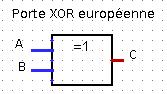
\includegraphics{images/porte_xor_european.png}\\

\end{minipage} &

\begin{minipage}{0.5\linewidth}

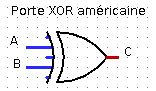
\includegraphics{images/porte_xor_american.png}\\

\end{minipage} \end{tabular}

\end{center}

\hypertarget{circuits-combinatoires}{%
\section{Circuits combinatoires}\label{circuits-combinatoires}}

\hypertarget{duxe9finition}{%
\subsection{Définition}\label{duxe9finition}}

\begin{definition}{}

Un \textbf{circuit logique combinatoire} permet de réaliser une ou
plusieurs fonctions booléennes : ses sorties ne dépendent que de l'état
actuel de ses entrées. Les portes logiques
\passthrough{\lstinline!NOT!}, \passthrough{\lstinline!NOR!},
\passthrough{\lstinline!NAND!}, \passthrough{\lstinline!AND!},
\passthrough{\lstinline!OR!} et \passthrough{\lstinline!XOR!} sont des
circuits combinatoires.

Il existe d'autres circuits, dits séquentiels, dont les sorties se
calculent non seulement à partir de leurs valeurs d'entrée actuelles
mais aussi à partir de leurs états précédents : le facteur temps
intervient. Ils utilisent des circuits de mémoire pour mémoriser leurs
états antérieurs.

\end{definition}

\begin{exercice}{}

On considère la fonction booléeenne \(f\) dont la table de vérité est
donnée ci-dessous :

\begin{longtable}[]{@{}cll@{}}
\toprule
\(x\) & \(y\) & \(f(x, y)\)\tabularnewline
\midrule
\endhead
0 & 0 & 1\tabularnewline
0 & 1 & 0\tabularnewline
1 & 0 & 0\tabularnewline
1 & 1 & 1\tabularnewline
\bottomrule
\end{longtable}

\begin{enumerate}
\def\labelenumi{\arabic{enumi}.}
\item
  En utilisant la méthode exposée dans l'exercice 8, déterminer une
  expression booléenne de la fonction \(f\).
\item
  Ouvrir le logiciel \href{http://www.cburch.com/logisim/}{Logisim} et
  construire un circuit combinatoire représentant cette fonction
  booléenne :

  \begin{itemize}
  \tightlist
  \item
    En utilisant les portes logiques \passthrough{\lstinline!NOT!},
    \passthrough{\lstinline!NOR!}, \passthrough{\lstinline!NAND!},
    \passthrough{\lstinline!AND!}, \passthrough{\lstinline!OR!} ou
    \passthrough{\lstinline!XOR!}.
  \item
    En n'utilisant que des portes logiques
    \passthrough{\lstinline!NOT!}, \passthrough{\lstinline!AND!} ou
    \passthrough{\lstinline!OR!}.
  \item
    En n'utilisant que des portes logiques
    \passthrough{\lstinline!NOR!}.
  \end{itemize}
\end{enumerate}

\href{videos/exercice9.mp4}{Tutoriel video : exercice 9}

\end{exercice}

\hypertarget{duxe9codeur-avec-2-bits-dentruxe9es}{%
\subsection{Décodeur avec 2 bits
d'entrées}\label{duxe9codeur-avec-2-bits-dentruxe9es}}

\begin{exercice}{}

On considère un circuit combinatoire qui possède deux entrées \(e_{0}\)
et \(e_{1}\) et quatre sorties \(s_{0}\), \(s_{1}\), \(s_{2}\) et
\(s_{3}\).

La sortie indexée par le nombre dont le bit de poids faible est
\(e_{0}\) et le bit de poids fort \(e_{1}\), est positionnée à \(1\) et
les autres sorties à \(0\). Ce circuit est ainsi appelé \textbf{décodeur
\(2\) bits}.

\begin{enumerate}
\def\labelenumi{\arabic{enumi}.}
\tightlist
\item
  Compléter la table de vérité de ce circuit combinatoire.
\end{enumerate}

\begin{longtable}[]{@{}clllll@{}}
\toprule
\(e_{0}\) & \(e_{1}\) & \(s_{0}\) & \(s_{1}\) & \(s_{2}\) &
\(s_{3}\)\tabularnewline
\midrule
\endhead
0 & 0 & & & &\tabularnewline
0 & 1 & & & &\tabularnewline
1 & 0 & & & &\tabularnewline
1 & 1 & & & &\tabularnewline
\bottomrule
\end{longtable}

\begin{enumerate}
\def\labelenumi{\arabic{enumi}.}
\setcounter{enumi}{1}
\item
  En utilisant la méthode exposée dans l'exercice 7, déterminer une
  expression booléenne de chacune des sorties \(s_{0}\), \(s_{1}\),
  \(s_{2}\) et \(s_{3}\), en fonction des entrées \(e_{0}\) et
  \(e_{1}\).
\item
  Ouvrir le logiciel \href{http://www.cburch.com/logisim/}{Logisim} et
  construire un circuit combinatoire représentant un \textbf{décodeur
  \(2\) bits}.
\end{enumerate}

\end{exercice}

\hypertarget{demi-additionneur-et-additionneur-1-bit}{%
\subsection{Demi-additionneur et additionneur 1
bit}\label{demi-additionneur-et-additionneur-1-bit}}

\begin{exercice}{}

\begin{enumerate}
\def\labelenumi{\arabic{enumi}.}
\item
  Effectuer les additions binaires : \(0+0\), \(0+1\), \(1+0\) et
  \(1+1\).
\item
  Un \textbf{demi-additionneur binaire 1 bit} est un circuit
  combinatoire qui possède :

  \begin{itemize}
  \tightlist
  \item
    deux entrées : deux bits d'opérande \(e_{0}\) et \(e_{1}\) ;
  \item
    deux sorties : un bit de résultat \(s\) et un bit de retenue
    sortante \(r\).
  \end{itemize}
\end{enumerate}

La sortie \(s\) prend pour valeur le bit des unités et la sortie \(r\)
le bit de retenue sortante, lorsqu'on additionne les deux bits d'entrée
\(e_{0}\) et \(e_{1}\).

\begin{enumerate}
\def\labelenumi{\arabic{enumi}.}
\tightlist
\item
  Compléter la table de vérité de ce circuit combinatoire :
\end{enumerate}

\begin{longtable}[]{@{}clll@{}}
\toprule
\(e_{0}\) & \(e_{1}\) & \(s\) & \(r\)\tabularnewline
\midrule
\endhead
0 & 0 & &\tabularnewline
0 & 1 & &\tabularnewline
1 & 0 & &\tabularnewline
1 & 1 & &\tabularnewline
\bottomrule
\end{longtable}

\begin{enumerate}
\def\labelenumi{\arabic{enumi}.}
\setcounter{enumi}{3}
\tightlist
\item
  Justifier qu'un \textbf{demi-additionneur binaire 1 bit} peut être
  représenté par le circuit ci-dessous.
\end{enumerate}

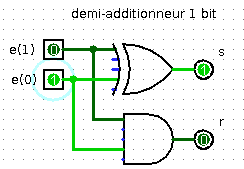
\includegraphics[width=0.5\textwidth,height=\textheight]{images/demi_additionneur.png}\\

\begin{enumerate}
\def\labelenumi{\arabic{enumi}.}
\setcounter{enumi}{4}
\tightlist
\item
  Ouvrir le logiciel \href{http://www.cburch.com/logisim/}{Logisim} et
  construire un circuit combinatoire représentant un
  \textbf{demi-additionneur binaire 1 bit}.
\end{enumerate}

\href{videos/exercice11.mp4}{Tutoriel video : exercice 11}

\end{exercice}

\begin{exercice}{}

Un \textbf{additionneur binaire 1 bit} est un circuit combinatoire qui
possède :

\begin{itemize}
\tightlist
\item
  trois entrées : deux bits d'opérande \(e_{0}\) et \(e_{1}\) et un bit
  de retenue entrante \(r_{0}\)
\item
  deux bits de sortie : un bit de résultat \(s_{2}\) et un bit de
  retenue sortante \(r_{3}\).
\end{itemize}

\begin{enumerate}
\def\labelenumi{\arabic{enumi}.}
\tightlist
\item
  Compléter les colonnes de la table de vérité d'un \textbf{additionneur
  binaire 1 bit} pour le bit de résultat \(s_{2}\) et le bit retenue
  sortante \(r_{3}\).
\end{enumerate}

\begin{longtable}[]{@{}clllllll@{}}
\toprule
\begin{minipage}[b]{0.05\columnwidth}\centering
\(e_{0}\)\strut
\end{minipage} & \begin{minipage}[b]{0.05\columnwidth}\raggedright
\(e_{1}\)\strut
\end{minipage} & \begin{minipage}[b]{0.05\columnwidth}\raggedright
\(r_{0}\)\strut
\end{minipage} & \begin{minipage}[b]{0.14\columnwidth}\raggedright
\(s_{1}=\ldots \ldots\)\strut
\end{minipage} & \begin{minipage}[b]{0.12\columnwidth}\raggedright
\(r_{1}=\ldots \ldots\)\strut
\end{minipage} & \begin{minipage}[b]{0.14\columnwidth}\raggedright
\(s_{2}=\ldots \ldots\)\strut
\end{minipage} & \begin{minipage}[b]{0.12\columnwidth}\raggedright
\(r_{2}=\ldots \ldots\)\strut
\end{minipage} & \begin{minipage}[b]{0.12\columnwidth}\raggedright
\(r_{3}=\ldots \ldots\)\strut
\end{minipage}\tabularnewline
\midrule
\endhead
\begin{minipage}[t]{0.05\columnwidth}\centering
0\strut
\end{minipage} & \begin{minipage}[t]{0.05\columnwidth}\raggedright
0\strut
\end{minipage} & \begin{minipage}[t]{0.05\columnwidth}\raggedright
0\strut
\end{minipage} & \begin{minipage}[t]{0.14\columnwidth}\raggedright
\strut
\end{minipage} & \begin{minipage}[t]{0.12\columnwidth}\raggedright
\strut
\end{minipage} & \begin{minipage}[t]{0.14\columnwidth}\raggedright
\strut
\end{minipage} & \begin{minipage}[t]{0.12\columnwidth}\raggedright
\strut
\end{minipage} & \begin{minipage}[t]{0.12\columnwidth}\raggedright
\strut
\end{minipage}\tabularnewline
\begin{minipage}[t]{0.05\columnwidth}\centering
0\strut
\end{minipage} & \begin{minipage}[t]{0.05\columnwidth}\raggedright
1\strut
\end{minipage} & \begin{minipage}[t]{0.05\columnwidth}\raggedright
0\strut
\end{minipage} & \begin{minipage}[t]{0.14\columnwidth}\raggedright
\strut
\end{minipage} & \begin{minipage}[t]{0.12\columnwidth}\raggedright
\strut
\end{minipage} & \begin{minipage}[t]{0.14\columnwidth}\raggedright
\strut
\end{minipage} & \begin{minipage}[t]{0.12\columnwidth}\raggedright
\strut
\end{minipage} & \begin{minipage}[t]{0.12\columnwidth}\raggedright
\strut
\end{minipage}\tabularnewline
\begin{minipage}[t]{0.05\columnwidth}\centering
1\strut
\end{minipage} & \begin{minipage}[t]{0.05\columnwidth}\raggedright
0\strut
\end{minipage} & \begin{minipage}[t]{0.05\columnwidth}\raggedright
0\strut
\end{minipage} & \begin{minipage}[t]{0.14\columnwidth}\raggedright
\strut
\end{minipage} & \begin{minipage}[t]{0.12\columnwidth}\raggedright
\strut
\end{minipage} & \begin{minipage}[t]{0.14\columnwidth}\raggedright
\strut
\end{minipage} & \begin{minipage}[t]{0.12\columnwidth}\raggedright
\strut
\end{minipage} & \begin{minipage}[t]{0.12\columnwidth}\raggedright
\strut
\end{minipage}\tabularnewline
\begin{minipage}[t]{0.05\columnwidth}\centering
1\strut
\end{minipage} & \begin{minipage}[t]{0.05\columnwidth}\raggedright
1\strut
\end{minipage} & \begin{minipage}[t]{0.05\columnwidth}\raggedright
0\strut
\end{minipage} & \begin{minipage}[t]{0.14\columnwidth}\raggedright
\strut
\end{minipage} & \begin{minipage}[t]{0.12\columnwidth}\raggedright
\strut
\end{minipage} & \begin{minipage}[t]{0.14\columnwidth}\raggedright
\strut
\end{minipage} & \begin{minipage}[t]{0.12\columnwidth}\raggedright
\strut
\end{minipage} & \begin{minipage}[t]{0.12\columnwidth}\raggedright
\strut
\end{minipage}\tabularnewline
\begin{minipage}[t]{0.05\columnwidth}\centering
0\strut
\end{minipage} & \begin{minipage}[t]{0.05\columnwidth}\raggedright
0\strut
\end{minipage} & \begin{minipage}[t]{0.05\columnwidth}\raggedright
1\strut
\end{minipage} & \begin{minipage}[t]{0.14\columnwidth}\raggedright
\strut
\end{minipage} & \begin{minipage}[t]{0.12\columnwidth}\raggedright
\strut
\end{minipage} & \begin{minipage}[t]{0.14\columnwidth}\raggedright
\strut
\end{minipage} & \begin{minipage}[t]{0.12\columnwidth}\raggedright
\strut
\end{minipage} & \begin{minipage}[t]{0.12\columnwidth}\raggedright
\strut
\end{minipage}\tabularnewline
\begin{minipage}[t]{0.05\columnwidth}\centering
0\strut
\end{minipage} & \begin{minipage}[t]{0.05\columnwidth}\raggedright
1\strut
\end{minipage} & \begin{minipage}[t]{0.05\columnwidth}\raggedright
1\strut
\end{minipage} & \begin{minipage}[t]{0.14\columnwidth}\raggedright
\strut
\end{minipage} & \begin{minipage}[t]{0.12\columnwidth}\raggedright
\strut
\end{minipage} & \begin{minipage}[t]{0.14\columnwidth}\raggedright
\strut
\end{minipage} & \begin{minipage}[t]{0.12\columnwidth}\raggedright
\strut
\end{minipage} & \begin{minipage}[t]{0.12\columnwidth}\raggedright
\strut
\end{minipage}\tabularnewline
\begin{minipage}[t]{0.05\columnwidth}\centering
1\strut
\end{minipage} & \begin{minipage}[t]{0.05\columnwidth}\raggedright
0\strut
\end{minipage} & \begin{minipage}[t]{0.05\columnwidth}\raggedright
1\strut
\end{minipage} & \begin{minipage}[t]{0.14\columnwidth}\raggedright
\strut
\end{minipage} & \begin{minipage}[t]{0.12\columnwidth}\raggedright
\strut
\end{minipage} & \begin{minipage}[t]{0.14\columnwidth}\raggedright
\strut
\end{minipage} & \begin{minipage}[t]{0.12\columnwidth}\raggedright
\strut
\end{minipage} & \begin{minipage}[t]{0.12\columnwidth}\raggedright
\strut
\end{minipage}\tabularnewline
\begin{minipage}[t]{0.05\columnwidth}\centering
1\strut
\end{minipage} & \begin{minipage}[t]{0.05\columnwidth}\raggedright
1\strut
\end{minipage} & \begin{minipage}[t]{0.05\columnwidth}\raggedright
1\strut
\end{minipage} & \begin{minipage}[t]{0.14\columnwidth}\raggedright
\strut
\end{minipage} & \begin{minipage}[t]{0.12\columnwidth}\raggedright
\strut
\end{minipage} & \begin{minipage}[t]{0.14\columnwidth}\raggedright
\strut
\end{minipage} & \begin{minipage}[t]{0.12\columnwidth}\raggedright
\strut
\end{minipage} & \begin{minipage}[t]{0.12\columnwidth}\raggedright
\strut
\end{minipage}\tabularnewline
\bottomrule
\end{longtable}

\begin{enumerate}
\def\labelenumi{\arabic{enumi}.}
\setcounter{enumi}{1}
\item
  Un \textbf{additionneur binaire 1 bit} peut être réalisé à l'aide de
  deux \textbf{demi-additionneurs binaires 1 bit} :

  \begin{itemize}
  \tightlist
  \item
    Le premier \textbf{demi-additionneur binaire 1 bit} prend en entrée
    les bits d'opérande \(e_{0}\) et \(e_{1}\) et retourne en sortie un
    bit de résultat intermédiaire \(s_{1}\) et un bit de retenue
    sortante intermédiaire \(r_{1}\). Donner une expression booléenne de
    \(s_{1}\) et \(r_{1}\) en fonction de \(e_{0}\) et \(e_{1}\).
  \item
    Le second \textbf{demi-additionneur binaire 1 bit} prend en entrée
    le bit de résultat \(s_{1}\) et le bit de retenue entrante \(r_{0}\)
    et retourne en sortie le bit de résultat final \(s_{2}\) et un bit
    de retenue sortante intermédiaire \(r_{2}\). Donner une expression
    booléenne de \(s_{2}\) et \(r_{2}\) en fonction de \(s_{1}\) et
    \(r_{0}\).
  \item
    Enfin, la retenue sortante \(r_{3}\) s'obtient à partir de la
    retenue sortante \(r_{1}\) du premier demi-additionneur et de la
    retenue sortante \(r_{2}\) du second. Donner une expression
    booléenne de \(r_{3}\) en fonction de \(r_{1}\) et \(r_{2}\).
  \end{itemize}

  Compléter les colonnes \(s_{1}\), \(r_{1}\) et \(r_{2}\) puis
  \(s_{2}\) et \(r_{3}\) de la table de vérité de l'\textbf{additionneur
  binaire à 1 bit}.
\item
  Avec le logiciel \href{http://www.cburch.com/logisim/}{Logisim} ouvrir
  le fichier contenant le demi-additionneur de l'exercice précédent.

  \begin{itemize}
  \tightlist
  \item
    Ajouter un nouveau circuit avec
    \passthrough{\lstinline!Add a circuit!} , le nommer
    \passthrough{\lstinline!additionneur1bit!} puis copier/coller dedans
    le circuit du \textbf{demi-additionneur binaire 1 bit}. Compléter le
    circuit pour obtenir un \textbf{additionneur binaire 1 bit}.
  \item
    Ajouter un nouveau circuit avec
    \passthrough{\lstinline!Add a circuit!} , le nommer
    \passthrough{\lstinline!additionneur2bits!} puis copier/coller
    dedans le circuit de l' \textbf{additionneur binaire 1 bit}.
    Compléter le circuit pour obtenir un \textbf{additionneur binaire 2
    bits}.
  \end{itemize}
\end{enumerate}

\href{videos/exercice12.mp4}{Tutoriel video : exercice 12}

\end{exercice}

\hypertarget{opuxe9rations-bit-uxe0-bit-en-python-hors-programme-de-premiuxe8re-nsi}{%
\section{\texorpdfstring{Opérations bit à bit en \texttt{Python} (hors
programme de première
NSI)}{Opérations bit à bit en Python (hors programme de première NSI)}}\label{opuxe9rations-bit-uxe0-bit-en-python-hors-programme-de-premiuxe8re-nsi}}

\begin{propriete}{}

Les fonctions booléennes élémentaires (\passthrough{\lstinline!OR!},
\passthrough{\lstinline!AND!}, \passthrough{\lstinline!NOT!},
\passthrough{\lstinline!XOR!}) existent en
\passthrough{\lstinline!Python!} sous la forme d'opérateurs booléens
mais sont également implémentés sous la forme d'opérateurs bit à bit sur
les nombres. Un \emph{opérateur bit à bit} (\emph{bitwise} en anglais)
s'applique sur les bits de même poids des représentations binaires de
ses opérandes.

\begin{longtable}[]{@{}lll@{}}
\toprule
\begin{minipage}[b]{0.24\columnwidth}\raggedright
Opérateur booléen\strut
\end{minipage} & \begin{minipage}[b]{0.22\columnwidth}\raggedright
Opérateur bit à bit\strut
\end{minipage} & \begin{minipage}[b]{0.46\columnwidth}\raggedright
Exemple\strut
\end{minipage}\tabularnewline
\midrule
\endhead
\begin{minipage}[t]{0.24\columnwidth}\raggedright
\passthrough{\lstinline!and!} , ET\strut
\end{minipage} & \begin{minipage}[t]{0.22\columnwidth}\raggedright
\passthrough{\lstinline!\&!}\strut
\end{minipage} & \begin{minipage}[t]{0.46\columnwidth}\raggedright
\passthrough{\lstinline!>>> bin(0b101001 \& 0b101010)!}\strut
\end{minipage}\tabularnewline
\begin{minipage}[t]{0.24\columnwidth}\raggedright
\strut
\end{minipage} & \begin{minipage}[t]{0.22\columnwidth}\raggedright
\strut
\end{minipage} & \begin{minipage}[t]{0.46\columnwidth}\raggedright
\passthrough{\lstinline!'0b101000'!}\strut
\end{minipage}\tabularnewline
\begin{minipage}[t]{0.24\columnwidth}\raggedright
\passthrough{\lstinline!or!} , OU\strut
\end{minipage} & \begin{minipage}[t]{0.22\columnwidth}\raggedright
\passthrough{\lstinline!|!}\strut
\end{minipage} & \begin{minipage}[t]{0.46\columnwidth}\raggedright
\passthrough{\lstinline!>>> bin(0b101001 | 0b101010)!}\strut
\end{minipage}\tabularnewline
\begin{minipage}[t]{0.24\columnwidth}\raggedright
\strut
\end{minipage} & \begin{minipage}[t]{0.22\columnwidth}\raggedright
\strut
\end{minipage} & \begin{minipage}[t]{0.46\columnwidth}\raggedright
\passthrough{\lstinline!'0b101011'!}\strut
\end{minipage}\tabularnewline
\begin{minipage}[t]{0.24\columnwidth}\raggedright
\passthrough{\lstinline!xor!} , OU EXCLUSIF\strut
\end{minipage} & \begin{minipage}[t]{0.22\columnwidth}\raggedright
\passthrough{\lstinline!^!}\strut
\end{minipage} & \begin{minipage}[t]{0.46\columnwidth}\raggedright
\passthrough{\lstinline!>>> bin(0b101001 ^ 0b101010)!}\strut
\end{minipage}\tabularnewline
\begin{minipage}[t]{0.24\columnwidth}\raggedright
\strut
\end{minipage} & \begin{minipage}[t]{0.22\columnwidth}\raggedright
\strut
\end{minipage} & \begin{minipage}[t]{0.46\columnwidth}\raggedright
\passthrough{\lstinline!'0b000011'!}\strut
\end{minipage}\tabularnewline
\begin{minipage}[t]{0.24\columnwidth}\raggedright
\passthrough{\lstinline!not!} , NEGATION\strut
\end{minipage} & \begin{minipage}[t]{0.22\columnwidth}\raggedright
\passthrough{\lstinline!\~!}\strut
\end{minipage} & \begin{minipage}[t]{0.46\columnwidth}\raggedright
\passthrough{\lstinline!>>> \~5 \#\~x retourne -x - 1!}\strut
\end{minipage}\tabularnewline
\begin{minipage}[t]{0.24\columnwidth}\raggedright
\strut
\end{minipage} & \begin{minipage}[t]{0.22\columnwidth}\raggedright
\strut
\end{minipage} & \begin{minipage}[t]{0.46\columnwidth}\raggedright
\passthrough{\lstinline!-6!}\strut
\end{minipage}\tabularnewline
\bottomrule
\end{longtable}

\end{propriete}

Exemples d'utilisation d'opérateurs bit à bit :

\begin{itemize}
\tightlist
\item
  On peut utiliser le \passthrough{\lstinline!ET!} bit à bit pour
  sélectionner uniquement certains bits, par exemple les bits de rang
  pairs :
\end{itemize}

\begin{lstlisting}[language=Python]
>>> bits_pairs = sum(2 ** k for k in range(0, 8, 2))
>>> bin(bits_pairs)
'0b1010101'
>>> bin(183)
'0b10110111'
>>> bin(183 & bits_pairs)
'0b10100010'
\end{lstlisting}

\begin{itemize}
\tightlist
\item
  Le \passthrough{\lstinline!OU EXCLUSIF!} peut servir à masquer /
  démasquer une partie de la représentation binaire d'un nombre (on peut
  l'employer avec tout objet codé numériquement comme une image ou un
  caractère).
\end{itemize}

\begin{lstlisting}[language=Python]
>>> diego = 69
>>> masque = 42
>>> zorro = diego ^ masque
>>> zorro
111
>>> zorro ^ masque
69
\end{lstlisting}

\begin{exercice}{}

Dans un réseau \passthrough{\lstinline!IP!} l'adresse
\passthrough{\lstinline!IP!} d'une machine est constituée d'un préfixe
correspondant à l'adresse du réseau (commune à toutes les machines du
réseau) et à un suffixe machine, identifiant la machine sur le réseau.

Le préfixe réseau s'obtient à partir de l'adresse
\passthrough{\lstinline!IP!} de la machine en faisant un
\passthrough{\lstinline!ET!} bit à bit avec le masque de sous-réseau.

Par exemple si l'adresse est \passthrough{\lstinline!192.168.11.12!} de
représentation binaire
\passthrough{\lstinline!11000000.10101000.00001011.00001011!} et le
masque de sous-réseau est \passthrough{\lstinline!255.255.252.0!} de
représentation binaire

\passthrough{\lstinline!11111111.11111111.11111100.00000000!} alors le
préfixe réseau est
\passthrough{\lstinline!11000000.10101000.00001000.00000000!} soit
\passthrough{\lstinline!192.168.8.0!}.

On donne ci-dessous deux fonctions outils :

\begin{lstlisting}[language=Python]
def ip2liste(ip):
    "Transforme une  adresse IP V4 (type str) en liste d'entiers"
    return [int(champ) for champ in ip.split('.')]

def liste2ip(ipliste):
    "Transforme une  liste d'entiers en adresse IP V4 (type str)"
    return '.'.join(str(n) for n in ipliste)
\end{lstlisting}

\begin{enumerate}
\def\labelenumi{\arabic{enumi}.}
\item
  Écrire une fonction de signature
  \passthrough{\lstinline!prefixe\_reseau(ip, masque)!} qui retourne le
  préfixe réseau sous forme d'adresse IP V4 (type
  \passthrough{\lstinline!str!}) à partir d'une adresse IP V4 et d'un
  masque de sous-réseau.
\item
  Écrire une fonction de signature
  \passthrough{\lstinline!suffixe\_machine(ip, masque)!} qui retourne le
  suffixe machine sous forme d'adresse IP V4 (type
  \passthrough{\lstinline!str!}) à partir d'une adresse IP V4 et d'un
  masque de sous-réseau.
\end{enumerate}

Voici un exemple de résultat attendu :

\begin{lstlisting}[language=Python]
>>> prefixe_reseau('145.245.11.254','255.255.252.0')
'145.245.8.0'
>>> suffixe_machine('145.245.11.254','255.255.252.0')
'0.0.3.254'
\end{lstlisting}

\end{exercice}

\begin{propriete}{}

\passthrough{\lstinline!Python!} définit également des opérateurs sur
les bits d'un nombre, plus efficaces que les opérations mathématiques
équivalentes :

\begin{itemize}
\item
  Le décalage de \passthrough{\lstinline!nombre!} de
  \passthrough{\lstinline!n!} bits vers la gauche multiplie
  \passthrough{\lstinline!nombre!} par \(2^{n}\) et s'écrit
  \passthrough{\lstinline!nombre << n!}.
\item
  Le décalage de \passthrough{\lstinline!nombre!} de
  \passthrough{\lstinline!n!} bits vers la droite divise
  \passthrough{\lstinline!nombre!} par \(2^{n}\) et s'écrit
  \passthrough{\lstinline!nombre >> n!}.
\end{itemize}

\end{propriete}

\begin{exercice}{}

Dans l'algorithme de recherche dichotomique, après division en deux de
la zone de recherche, l'algorithme s'appelle lui-même sur l'une des deux
moitiés. C'est un algorithme de type \emph{Diviser pour régner} qui peut
se programmer récursivement comme nous le verrons en terminale dans le
chapitre sur la récursivité.

Si on note \emph{n} la taille de la liste, une autre implémentation, non
récursive, est la suivante :

\begin{itemize}
\item
  on commence la recherche au début de la liste et on avance avec un pas
  \passthrough{\lstinline!pas = n // 2!} ou
  \passthrough{\lstinline!pas = n >> 1!} jusqu'au premier élément
  supérieur à l'élément cherché ;
\item
  on repart de l'élément précédent le point d'arrêt et on avance
  désormais avec un pas divisé par 2 soit :

  \passthrough{\lstinline!pas = pas >> 1!} ;
\item
  on répète en boucle ces instructions jusqu'à ce que le pas atteigne
  \(1\).
\end{itemize}

A la fin de de la boucle, on détermine si l'élément précédent le dernier
point d'arrêt est l'élément recherché.

Compléter le code de la fonction
\passthrough{\lstinline!recherche\_dicho2!} qui implémente cet
algorithme.

\begin{lstlisting}[language=Python]
def recherche_dicho2(L, e):
    x, n  = 0, len(L)
    pas = n >> 1
    while pas >= 1:
        while x + pas < n and .................:
            x = ..............
        pas = ................
    return ............
\end{lstlisting}

\end{exercice}

\end{document}
